\setcounter{dang}{0}
\section{PHƯƠNG TRÌNH, BẤT PHƯƠNG TRÌNH MŨ VÀ LOGARIT}
\subsection{Lý thuyết cần nhớ}
\subsubsection{Công thức nghiệm của phương trình mũ}
\begin{itemize}
\item [\faCheckSquareO]Dạng \fbox{$a^x=b$} (1), với $a>0$ và $a \ne 1$.
	\item [\faCheckSquareO] Về mặt đồ thị, nghiệm của (1) là hoành độ giao điểm của đồ thị $y=a^x$ với đường thẳng $y=b$ (nằm ngang). 
	\immini{Từ hình vẽ, ta có các kết quả sau:
			\begin{listEX}[1]
				\item [\ding{172}] $b>0$ (1) có nghiệm duy nhất $x=\log_ab$.
				\item [\ding{173}] $b\le 0$ (1) vô nghiệm.
			\end{listEX}
		}{	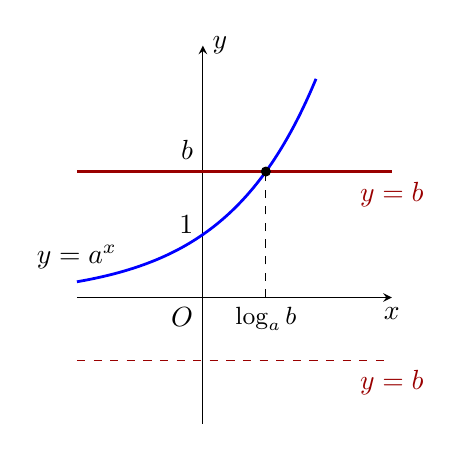
\begin{tikzpicture}[smooth,samples=300,scale=0.8,>=stealth]
		\draw[->] (-2,0)--(3,0) node[below]{$x$};
		\draw[->] (0,-2)--(0,4) node[right]{$y$};
		\draw (0,0) node[below left]{$O$};
		\draw[line width=1pt,color=blue,domain=-2:1.8] plot(\x,{2^(\x)});
		\draw[color=red!60!black,line width=1pt] (-2,2)--(3,2) node[below]{$y=b$};
		\draw[dashed,color=red!60!black] (-2,-1)--(3,-1) node[below]{$y=b$};
		\draw[dashed] (1,0)node[below]{\small$\log_ab$}--(1,2);
		\draw[fill=black](1,2) circle(2pt);
		\node[above] at (-2,0.3) {$y=a^x$};
		\node[left] at (0,2.35) {$b$};
		\node[left] at (0,1.15) {$1$};
		\end{tikzpicture}}
\begin{khung4}{GHI NHỚ}
	Với $a>0$ và $a \ne 1$, $b>0$, ta có các công thức sau đây: 
	\begin{listEX}[2]
		\item [\ding{172}] $a^{f(x)}=b \Leftrightarrow f(x)=\log_ab$
		\item [\ding{173}] $a^{f(x)}=a^{g(x)} \Leftrightarrow f(x)=g(x)$
	\end{listEX}
\end{khung4}
\end{itemize}
\subsubsection{Công thức nghiệm của phương trình lôgarit}
\begin{itemize}
\item [\faCheckSquareO]Dạng \fbox{$\log_ax=b$} (2), với $a>0$ và $a \ne 1$.
		\item [\faCheckSquareO]Về mặt đồ thị, nghiệm của (2) là hoành độ giao điểm của đồ thị $y=\log_ax$ với đường thẳng $y=b$ (nằm ngang). 
	\immini{	
		Từ hình vẽ, ta có các kết quả sau:
		\begin{listEX}[1]
				\item [\ding{172}] Với mọi $b$, (2) luôn có nghiệm duy nhất.
				\item [\ding{173}] $\log_ax=b \Leftrightarrow x=a^b$.
			\end{listEX}
		}{	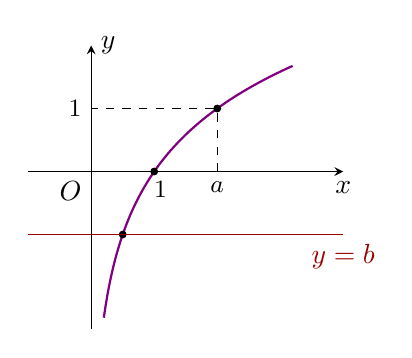
\begin{tikzpicture}[smooth,samples=300,scale=0.8,>=stealth]
			\draw[->] (-1,0)--(4,0) node[below]{$x$};
			\draw[->] (0,-2.5)--(0,2) node[right]{$y$};
			\draw (0,0) node[below left]{$O$};
			\draw[line width=0.8pt,color=violet,domain=0.2:3.2]plot(\x,{ln((\x))/ln(2)});
			\draw[fill=black] (1,0) circle(1.5pt) (2,1) circle(1.5pt) (0.5,-1) circle(1.5pt);
			\draw[dashed] (2,0)node[below]{\small$a$}--(2,1)--(0,1)node[left]{\small$1$};
			\draw[color=red!60!black] (-1,-1)--(4,-1) node[below]{$y=b$};
			\node[below] at (1.1,0) {\small$1$};
			\end{tikzpicture}}
		
\begin{khung4}{GHI NHỚ}
	Với $a>0$ và $a \ne 1$, $b$ bất kì, ta có các công thức sau đây: 
	\begin{listEX}[1]
		\item [\ding{172}] $\log_ax=b \Leftrightarrow x=a^b$.
		\item [\ding{173}] $\log_a{f(x)}=\log_a{g(x)}\Leftrightarrow \heva{&f(x)>0 \,(\text{ hoặc } g(x)>0)\\&f(x)=g(x)}$.
	\end{listEX}
\end{khung4}
\end{itemize}

\subsubsection{Công thức nghiệm của bất phương trình mũ}
Minh họa dạng \fbox{$a^x>b$}, với $a>0$ và $a \ne 1$.\\
\hspace*{1cm}
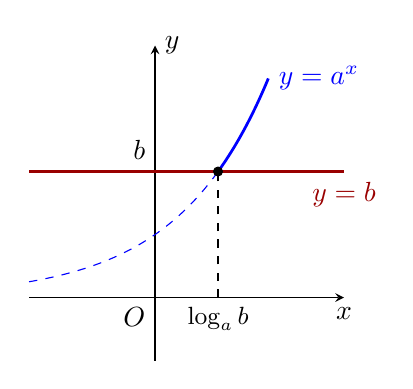
\begin{tikzpicture}[smooth,samples=300,scale=0.8,>=stealth]
	\draw[->] (-2,0)--(3,0) node[below]{$x$};
	\draw[->] (0,-1)--(0,4) node[right]{$y$};
	\draw (0,0) node[below left]{$O$};
	\draw[dashed,color=blue,domain=-2:1] plot(\x,{2^(\x)});
	\draw[line width=1pt,color=blue,domain=1:1.8] plot(\x,{2^(\x)})node[right]{$y=a^x$};
	\draw[color=red!60!black,line width=1pt] (-2,2)--(3,2) node[below]{$y=b$};
	\draw[dashed] (1,0)node[below]{\small$\log_ab$}--(1,2);
	\draw[fill=black](1,2) circle(2pt);
	\node[left] at (0,2.35) {$b$};
\end{tikzpicture}
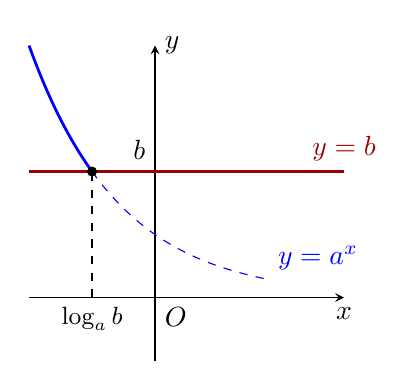
\begin{tikzpicture}[smooth,samples=300,scale=0.8,>=stealth]
	\draw[->] (-2,0)--(3,0) node[below]{$x$};
	\draw[->] (0,-1)--(0,4) node[right]{$y$};
	\draw (0,0) node[below right]{$O$};
	\draw[dashed,color=blue,domain=-1:1.8] plot(\x,{0.5^(\x)})node[above right]{$y=a^x$};
	\draw[line width=1pt,color=blue,domain=-2:-1] plot(\x,{0.5^(\x)});
	\draw[color=red!60!black,line width=1pt] (-2,2)--(3,2) node[above]{$y=b$};
	\draw[dashed] (-1,0)node[below]{\small$\log_ab$}--(-1,2);
	\draw[fill=black](-1,2) circle(2pt);
	\node[left] at (0,2.35) {$b$};
\end{tikzpicture}
\begin{itemize}
	\item [$\bullet$] Nếu $b \le 0$ thì tập nghiệm của bất phương trình là $\mathbb{R}$.
	\item [$\bullet$] Nếu $b>0$, ta có hai trường hợp:
		\begin{listEX}[1]
			\item [\ding{172}] Với $a>1$ thì \fbox{$a^x>b \Leftrightarrow x>\log_ab$} (Hình bên trái).
			\item [\ding{173}] Với $0<a<1$ thì \fbox{$a^x>b \Leftrightarrow x<\log_ab$} (Hình bên phải).
		\end{listEX}
\end{itemize}
\subsubsection{Công thức nghiệm của bất phương trình lôgarit}
Minh họa dạng \fbox{$\log_ax>b$}, với $a>0$ và $a \ne 1$.\\
\begin{center}
	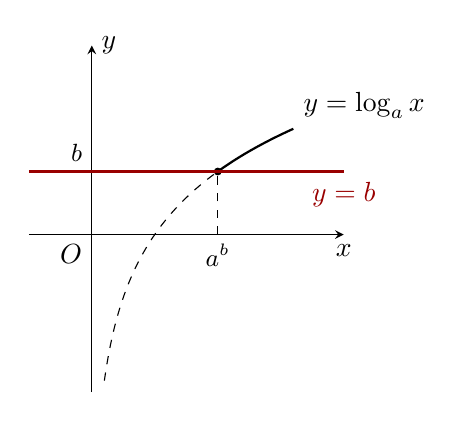
\begin{tikzpicture}[smooth,samples=300,scale=0.8,>=stealth]
	\draw[->] (-1,0)--(4,0) node[below]{$x$};
	\draw[->] (0,-2.5)--(0,3) node[right]{$y$};
	\draw (0,0) node[below left]{$O$};
	\draw[dashed,black,domain=0.2:2]plot(\x,{ln((\x))/ln(2)});
	\draw[line width=0.8pt,black,domain=2:3.2]plot(\x,{ln((\x))/ln(2)})node[above right]{$y=\log_ax$};
	\draw[fill=black] (2,1) circle(1.5pt);
	\draw[dashed] (2,0)node[below]{\small$a^b$}--(2,1)--(0,1)node[above left]{\small$b$};
	\draw[color=red!60!black,thick] (-1,1)--(4,1) node[below]{$y=b$};
\end{tikzpicture}
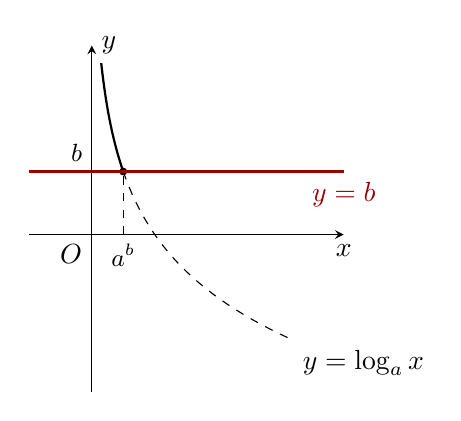
\begin{tikzpicture}[smooth,samples=300,scale=0.8,>=stealth]
	\draw[->] (-1,0)--(4,0) node[below]{$x$};
	\draw[->] (0,-2.5)--(0,3) node[right]{$y$};
	\draw (0,0) node[below left]{$O$};
	\draw[dashed,black,domain=0.5:3.2]plot(\x,{ln((\x))/ln(0.5)})node[below right]{$y=\log_ax$};
	\draw[line width=0.8pt,black,domain=0.15:0.5]plot(\x,{ln((\x))/ln(0.5)});
	\draw[fill=black] (0.5,1) circle(1.5pt);
	\draw[dashed] (0.5,0)node[below]{\small$a^b$}--(0.5,1)--(0,1)node[above left]{\small$b$};
	\draw[color=red!60!black,thick] (-1,1)--(4,1) node[below]{$y=b$};
\end{tikzpicture}
\end{center}

\begin{itemize}
	\item [$\bullet$] Điều kiện xác định là $x>0$.
	\item [$\bullet$] Ta có hai trường hợp:
		\begin{listEX}[1]
			\item [\ding{172}] Với $a>1$ thì \fbox{$\log_ax>b \Leftrightarrow x>a^b$} (Hình bên trái).
			\item [\ding{173}] Với $0<a<1$ thì \fbox{$\log_ax>b \Leftrightarrow 0<x<a^b$} (Hình bên phải).
		\end{listEX}
\end{itemize}
\begin{khung4}{Ghi nhớ}
	Các trường hợp $a^x \ge b$, $a^x<b$, $a^x \le b$, $\log_ax \ge b$, $\log_ax < b$, $\log_ax \le b$... ta suy luận tương tự.
		\begin{itemize}
			\item [$\bullet$] Cơ số $a> 1$: Ta so sánh "cùng chiều";
			\item [$\bullet$] Cơ số $0<a<1$: Ta so sánh "nghịch chiều".
		\end{itemize}
	Khi giải phương trình hoặc bất phương trình logarit, ta cần chú ý đặt điều kiện để các biểu thức logarit có nghĩa trước khi biến đổi (nếu không chắc phép biến đổi đó là phép biến đổi tương đương)
\end{khung4}
\subsection{Các dạng toán thường gặp}

\begin{dang}{Giải các phương trình mũ và logarit đơn giản}
\end{dang}

\begin{vd}
	Giải các phương trình mũ sau:
	\begin{enumEX}[a)]{1}
		\item $2^x=3$;
		\item $2^{x-1}=32$;
		\item $5^{x^2-5x-6} = 1$;
		\item $4^{2x+5}=2^{2-x}$;
		\item $3^{x-4} = \left(\dfrac{1}{9}\right)^{3x-1}$;
		\item $(0,4)^{8-2x^2}=(6,25)^{3x}$;
		\item $\left(\dfrac{1}{25}\right)^{x-1}=125^{2x}$;
		\item $2^x\cdot 3^{x-1}\cdot 5^{x-2}=12$;
		\item $2^x\cdot 15^{x+1}=3^{x+3}$.
	\end{enumEX}
	\loigiai{
		\begin{enumerate}[a)]
			\item Ta có ${2}^{x}=3 \Leftrightarrow x=\log_{2}{3}$.
			\item Ta có $2^{x-1}=32\Leftrightarrow x-1=\log_2 32\Leftrightarrow x-1=5\Leftrightarrow x=6$.\\
			Vậy phương trình có nghiệm là $x=6$.
			\item $5^{x^2-5x-6} = 1 \Leftrightarrow x^2 - 5x - 6 = 0 \Leftrightarrow \hoac{& x = -1 \\& x = 6.}$
			\item Ta có
			$$4^{2x+5}=2^{2-x}\Leftrightarrow 2^{2(2x+5)}=2^{2-x}\Leftrightarrow 2(2x+5)=2-x\Leftrightarrow x=-\dfrac{8}{5}.$$
			Vậy, nghiệm của phương trình là $x=-\dfrac{8}{5}$.	
			\item Ta có $3^{x-4} = \left(\dfrac{1}{9}\right)^{3x-1} \Leftrightarrow 3^{x - 4} = 3^{-6x+2} \Leftrightarrow x - 4 = -6x+2 \Leftrightarrow x = \dfrac{6}{7}$.
			\item Ta có
			$$(0,4)^{8-2x^2}=(6,25)^{3x}\Leftrightarrow \left(\dfrac{2}{5} \right) ^{8-2x^2}=\left(\dfrac{25}{4} \right)^{3x}\Leftrightarrow \left(\dfrac{5}{2} \right) ^{2x^2-8}=\left(\dfrac{5}{2} \right)^{6x}\Leftrightarrow 2x^2-8=6x \Leftrightarrow \hoac{&x=-1\\&x=4.}$$
			\item Ta có $\left(\dfrac{1}{25}\right)^{x-1}=125^{2x} \Leftrightarrow 5^{2-2x}=5^{6x} \Leftrightarrow 2-2x=6x \Leftrightarrow x=\dfrac{1}{4}$.
			\item Ta có  $2^x\cdot 3^{x-1}\cdot 5^{x-2}=12\Leftrightarrow 2^{x-2}\cdot 3^{x-2}\cdot 5^{x-2}=1\Leftrightarrow 30^{x-2}=1\Leftrightarrow x-2=0\Leftrightarrow x=2$.
			\item Ta có:  
			\begin{eqnarray*}
				&&2^x\cdot 15^{x+1}=3^{x+3}\\
				&\Leftrightarrow& 15\cdot 30^x=27\cdot 3^x\\
				&\Leftrightarrow& 10^x=\dfrac{9}{5}\\
				&\Leftrightarrow& x=\log \dfrac{9}{5}
			\end{eqnarray*}
	\end{enumerate}}
\end{vd} \dongcham{30}

\begin{vd}
	Giải các phương trình lôgarit sau:
	\begin{enumEX}[a)]{1}
		\item $\log {\left( x-1 \right) }=2$
		\item $\log_2\left(x^2-19x+2\right)=9$
		\item $\log_{0{,25}}(x^2+3x)=-1 $
		\item $\log_2 {\left(x^2-4x+3 \right)}=\log_2 {\left(4x-4 \right)}$
		\item $2\log_2x=\log_2(2-x)$ 
		\item $ \ln x+ \ln (3x-2)=0$
		\item $\ln(x+1)+\ln(x+3)=\ln(x+7)$ 
		\item $\log_2x+\log_2(x+2)=3$
		\item  $\log_3(2x+1)-\log_3(x-1)=1$.
		\item $\log_2\left(x^2 - 3\right) - \log_2(6x - 10) + 1 = 0$
		\item $2\log_{4}{x}+\log_{2}\left(x-3\right)=2$
		\item $\log_3 (x^2 + 4x) + \log_{\tfrac{1}{3}} (2x+3) = 0$ 
		
	\end{enumEX}
	\loigiai{
		\begin{enumerate}[a)]
			\item Điều kiện $x-1>0$ $\Leftrightarrow x>1$.\\
			Phương trình đã cho tương đương với
			\begin{eqnarray*}
				&&x-1=10^2 \\
				&\Leftrightarrow &x=101.
			\end{eqnarray*}
			\item Phương trình tương đương với $x^2-19x+2=2^9\Leftrightarrow x^2-19x-510=0\hoac{&  x=34 \\ & x=-15.}$
			\item Ta có
			$$\log_{0{,25}}(x^2+3x)=-1\Leftrightarrow x^2+3x=4\Leftrightarrow x^2+3x-4=0\Leftrightarrow\hoac{&x=1\\&x=-4.}$$
			\item Phương trình tương đương với
			\begin{eqnarray*}
				&&\heva{& x^2-4x+3=4x-4 \\ & 4x-4>0 }\\
				&\Leftrightarrow& \heva{& x^2-8x+7=0 \\ & x>1 }\\
				&\Leftrightarrow &\heva{& \hoac{&x=1 & (\textrm{loại}) \\ & x=7} \\ & x>1 }\\
				&\Leftrightarrow &x=7.
			\end{eqnarray*}
			\item Ta có $2\log_2x=\log_2(2-x)\Leftrightarrow \heva{
				& 0<x<2 \\
				& x^2=2-x \\}\Leftrightarrow \heva{
				& 0<x<2 \\
				& \hoac{
					& x=1 \\
					& x=-2 \\} \\}\Leftrightarrow x=1$.
				\item Điều kiện: $x> \dfrac{2}{3}$. \\
			Ta có $ \ln x+ \ln (3x-2)=0 \Leftrightarrow x(3x-2)=1 \Leftrightarrow 3x^2-2x-1=0 \Leftrightarrow \left[\begin{aligned}
				&x=1&&(\text{nhận}) \\
				&x=- \dfrac{1}{3}&&(\text{loại})
			\end{aligned} \right. $ \\
			Vậy phương trình $ \ln x+ \ln (3x-2)=0$ có $1$ nghiệm duy nhất.
			\item Điều kiện $x>-1$.\\
			Phương trình tương đương với
			\begin{eqnarray*}
				& &\ln\left[(x+1)(x+3)\right]=\ln(x+7)\\
				&\Leftrightarrow &(x+1)(x+3)=x+7\\
				&\Leftrightarrow & x^2+3x-4=0\Leftrightarrow \hoac{& x=1\text{ (thỏa mãn)} \\ & x=-4\text{ (loại)}.}
			\end{eqnarray*}
			Vậy phương trình có $1$ nghiệm.
			\item Điều kiện: $ x>0 $. \\
			Phương trình trở thành $$ \log_2 \left(x^2+2x\right) = 3 \Leftrightarrow x^2 + 2x - 8 = 0 \Leftrightarrow \hoac{&x=2\\&x=-4.} $$
			So với điều kiện $ x>0 $, phương trình đã cho có nghiệm duy nhất $ x = 2 $.
			\item Điều kiện $x>1$.\\ Phương trình tương đương với $\log_3\dfrac{2x+1}{x-1}=1\Leftrightarrow \dfrac{2x+1}{x-1}=3\Leftrightarrow 2x+1=3x-3\Rightarrow x=4$
			\item Điều kiện $\heva{& x^2-3>0 \\ & 6x-10>0.}$\\
			Khi đó, phương trình đã cho tương đương với $$\log_22(x^2-3)=\log_2 (6x-10)\Leftrightarrow2x^2-6x+4=0\Leftrightarrow\hoac{& x=1 \\ & x=2.}$$
			Thử lại, chỉ có $x=2$ thỏa mãn điều kiện.\\
			Vậy phương trình đã cho có một nghiệm.
			\item Điều kiện $\heva{&x>0\\&x-3>0} \Leftrightarrow x>3$.\\
			Phương trình đã cho tương đương với
			\begin{eqnarray*}
				&  & 2\log_{2^2}{x}+\log_{2}\left(x-3\right)=2\\
				& \Leftrightarrow & \log_{2}{x}+\log_{2}\left(x-3\right)=2\\
				& \Leftrightarrow & \log_{2}\left[x\left(x-3\right)\right]=2\\
				& \Leftrightarrow & x\left(x-3\right)={2}^{2}=4\\
				& \Leftrightarrow &  x^2-3x-4=0\\
				& \Leftrightarrow & \hoac{&x=4\\&x=-1.}
			\end{eqnarray*}
			So với điều kiện, nghiệm là $x=4$.
			\item Điều kiện $\heva{&x^2+4x>0\\ &2x+3>0}\Leftrightarrow x>0$.\\
			Phương trình tương đương với
			\begin{align*}
				&\ \log_3(x^2+4x)=\log_3(2x+3)\Leftrightarrow x^2+4x=2x+3\\
				\Leftrightarrow &\ x^2+2x-3=0\Leftrightarrow \hoac{&x=-3\\ &x=1.}
			\end{align*}
			Đối chiếu điều kiện, ta thấy $x=1$ là nghiệm của phương trình.
	\end{enumerate}}
\end{vd} \dongcham{30}

\begin{dang}{Giải các bất phương trình mũ và lôgarit đơn giản}
\end{dang}
\begin{vd}
	Giải các bất phương trình mũ sau:
	\begin{enumEX}[a)]{2}
		\item $3^{x-1}>1$;
		\item $ \left( \dfrac{1}{2}\right)^x \geq 2$;
		\item $\left(\dfrac{1}{2}\right)^{x^2-4x}<8$
		\item $(0,125)^{x^2}>\left(\dfrac{1}{8}\right)^{5x-6}$
		\item $\left(\dfrac{3}{4}\right)^{x-12}\ge \left(\dfrac{4}{3}\right)^x$
		\item $4^x>2^{x+8}$;
		\item $3^{2x + 1} > \left(\dfrac{1}{3}\right)^{- 3x^2}$;
		\item $\left(\dfrac{1}{2}\right)^{9x^2-17x+11} \geq \left(\dfrac{1}{2}\right)^{7-5x}$;
	\end{enumEX}
	\loigiai{
		\begin{enumerate}[a)]
			\item Ta có $3^{x-1}>1\Leftrightarrow x-1>0\Leftrightarrow x>1$.
			\item Ta có $ \left( \dfrac{1}{2}\right)^x \geq 2 \Leftrightarrow 2^{-x} \geq 2 \Leftrightarrow -x \geq 1\Leftrightarrow x\leq -1$.\\
			Vậy tập nghiệm của bất phương trình đã cho là $( -\infty; -1]$.
			\item Bất phương trình $\Leftrightarrow 2^{-x^2+4x}<2^3\Leftrightarrow -x^2+4x<3\Leftrightarrow x^2-4x+3>0\Leftrightarrow \hoac{& x>3\\ &x<1.}$
			\item Ta có: $(0,125)^{x^2}>\left(\dfrac{1}{8}\right)^{5 x-6}\Leftrightarrow\left(\dfrac{1}{8}\right)^{x^2}>\left(\dfrac{1}{8}\right)^{5 x-6}\Leftrightarrow x^2<5 x-6\Leftrightarrow x^2-5 x+6<0\Leftrightarrow 2<x<3$.\\
			Vậy tập nghiệm là $(2;3)$.
			\item Ta có $\left(\dfrac{3}{4}\right)^{x-12}\ge \left(\dfrac{4}{3}\right)^x\Leftrightarrow \left(\dfrac{4}{3}\right)^{12-x}\ge \left(\dfrac{4}{3}\right)^x\Leftrightarrow 12-x\ge x\Leftrightarrow x\le 6$. \\
			Vậy nghiệm lớn nhất của bất phương trình là $6$.
			\item Ta có $4^x>2^{x+8} \Leftrightarrow 2^{2x}>2^{x+8} \Leftrightarrow 2x>x+8 \Leftrightarrow x>8$
			\item Ta có
			$$3^{2x + 1} > \left(\dfrac{1}{3}\right)^{- 3x^2}\Leftrightarrow 3^{2x + 1} > 3^{3x^2}\Leftrightarrow 2x + 1 > 3x^2\Leftrightarrow 3x^2 - 2x - 1 < 0\Leftrightarrow -\dfrac{1}{3} < x < 1$$
			Vậy tập nghiệm của bất phương trình là $\left(- \dfrac{1}{3}; 1\right)$.
			\item \begin{eqnarray*}
				\left(\dfrac{1}{2}\right)^{9x^2-17x+11} \geq \left(\dfrac{1}{2}\right)^{7-5x} &\Leftrightarrow& 9x^2-17x+11 \leq 7-5x \Leftrightarrow 9x^2-12x+4 \leq 0 \\
				&\Leftrightarrow& \left(x-\dfrac{2}{3}\right)^2 \leq 0 \Leftrightarrow x=\dfrac{2}{3}.
			\end{eqnarray*}
		\end{enumerate}}
\end{vd} \dongcham{29}

\begin{vd}
	Giải các bất phương trình lôgarit sau:
	\begin{enumEX}[a)]{1}
		\item $\log x\ge 1$ 
		\item $\log_2 (3x-1)>3$ 
		\item $\log_{\tfrac{1}{2}}(x-3)\ge\log_{\tfrac{1}{2}} 4$
		\item  $\log_4(x+7)>\log_2(x+1)$
		\item $\log_2 (x^2 - x - 2) \leq 2\log_2 (3 - x)$
		\item  $ 2\log_2(x-1)>\log_2 (5-x)+1 $
	\end{enumEX}
	\loigiai{
		\begin{enumerate}[a)]
			\item Ta có $\log x\ge 1\Leftrightarrow x\ge 10$.\\
			Vậy tập nghiệm của bất phương trình là $[10:+\infty)$.
			\item $\log_2 (3x-1)>3\Leftrightarrow 3x-1>2^3\Leftrightarrow 3x>9\Leftrightarrow x>3$.
			\item Ta có: $\log_{\tfrac{1}{2}}(x-3)\ge{\log_{\tfrac{1}{2}}}4 $$\Leftrightarrow\heva{&x-3 > 0\\&x-3\le 4}$ $\Leftrightarrow\heva{&x > 3\\&x\le 7.}$\\
			Tập nghiệm của bất phương trình là $S=(3;7]$.
				\item Xét phương trình $\log_2 (x^2 - x - 2) \leq 2\log_2 (3 - x)$. \hfill (1)\\
			Ta có $(1) \Leftrightarrow \heva{&x^2 - x - 2 > 0\\&3 - x > 0\\&x^2 - x - 2 \leq x^2 - 6x + 9} \Leftrightarrow \heva{&\hoac{&x < -1\\&x > 2}\\&x < 3\\&x \leq \dfrac{11}{5}} \Leftrightarrow \hoac{&x < -1\\&2 < x \leq \dfrac{11}{5}.}$\\
			Vậy tập nghiệm của bất phương trình là $S = (-\infty; -1) \cup \left(2; \dfrac{11}{5}\right]$.
			\item Điều kiện: $x>-1$.
			\allowdisplaybreaks
			\begin{eqnarray*}
				&&\log_4(x+7)>\log_2(x+1)\Leftrightarrow\dfrac{1}{2}\log_2(x+7)>\log_2(x+1)\\
				&\Leftrightarrow& \heva{&x+1>0\\&\sqrt{x+7}>x+1}\Leftrightarrow \heva{&x>-1\\&x+7>(x+1)^2}\Leftrightarrow \heva{&x>-1\\&x^2+x-6<0}\\
				&\Leftrightarrow& \heva{&x>-1\\&-3<x<2}\Leftrightarrow x \in (-1;2).
			\end{eqnarray*}
			\item Điều kiện $ 1<x<5 $. Ta có
			\begin{align*}
				& 2\log_2(x-1)
				>\log_2 (5-x)+1\\
				\Leftrightarrow
				&\log_2 \left( x-1\right) ^2
				>\log_2\left( 2 (5-x)\right) \\
				\Leftrightarrow
				& (x-1)^2>2(5-x)\\
				\Leftrightarrow
				& x^2-9>0 \Leftrightarrow x<-3\cup x>3.
			\end{align*}
			Kết hợp với điều kiện bài toán, suy ra bất phương trình có tập nghiệm $ S=(3;5). $
	\end{enumerate}}
\end{vd} \dongcham{35}

\begin{dang}{Vận dụng, thực tiễn}
\end{dang}

\begin{vd}%[1C6Y3-4] 6.36
	Áp suất khí quyển $p$ lên một vật giảm khi độ cao tăng dần. Giả sử áp suất này (tính bằng milimét thuỷ ngân) được biểu diễn theo độ cao $h$ (tính bằng kilômét) so với mực nước biển bằng công thức $p(h)=760 \cdot \mathrm{e}^{-0,145 h}$.
	\begin{enumerate}
		\item Một máy bay đang chịu áp suất khí quyển $320$ $\mathrm{mmHg}$. Tìm độ cao của máy bay đó.
		\item Một người đứng trên đỉnh của một ngọn núi và chịu áp suất khí quyển $667$ $ \mathrm{mmHg}$. Tìm chiều cao của ngọn núi này.
	\end{enumerate}
	\loigiai{	
		\begin{enumerate}
			\item Giải phương trình $760 \mathrm{e}^{-0,145 h}=320$, ta tìm được $h \approx 5,965 \mathrm{~km}$.
			Vậy độ cao của máy bay là khoảng $5,965 \mathrm{~km}$.
			\item Giải phương trình $760 \mathrm{e}^{-0,145 h}=667$, ta tìm được $h \approx 0,9 \mathrm{~km}$.
			Vậy chiều cao của ngọn núi là khoảng $0,9 \mathrm{~km}$.
		\end{enumerate}
	}	
\end{vd} \dongcham{14}

\begin{vd}%[1D4G4-6]
	Đồng vị phóng xạ Uranium-$235$ (thường được sử dụng trong điện hạt nhân) có chu kì bán rã là $T=703800000$ năm. Theo đó, nếu ban đầu có $100$ gam Uranium-$235$ thì sau $t$ năm, do bị phân rã, lượng Uranium-$235$ còn lại được tính bởi công thức $M=100\left(\dfrac{1}{2}\right)^{\frac{t}{T}}$ (g). Sau thời gian bao lâu thì lượng Uranium-$235$ còn lại bằng $90 \%$ so với ban đầu?
	\loigiai{
		Khi $M=90$ g thì ta có phương trình
		\allowdisplaybreaks
		\begin{eqnarray*}
			90=100\left(\dfrac{1}{2}\right)^{\frac{t}{T}} 
			&\Leftrightarrow &\left(\dfrac{1}{2}\right)^{\frac{t}{T}}=0{,}9\\
			&\Leftrightarrow &\dfrac{t}{T}=\log _{\frac{1}{2}} 0{,}9\\
			&\Leftrightarrow &t=T \cdot \log _{\frac{1}{2}} 0{,}9 \approx 106979777 \ \text{năm}.
		\end{eqnarray*}
	}
\end{vd} \dongcham{14}

\begin{vd}%[1D4G4-6]
	Người ta dùng thuốc để khử khuẩn cho một thùng nước. Biết rằng nếu lúc đầu mỗi mililít nước chứa $P_{0}$ vi khuẩn thì sau $t$ giờ (kể từ khi cho thuốc vào thùng), số lượng vi khuẩn trong mỗi mililít nước là $P=P_0 \cdot 10^{-\alpha t}$, với $\alpha$ là một hằng số dương nào đó. Biết rằng ban đầu mỗi mililít nước có $9000$ vi khuẩn và sau $2$ giờ, số lượng vi khuẩn trong mỗi mililit nước là $6000$. Sau thời gian bao lâu thì số lượng vi khuẩn trong mỗi mililit nước trong thùng ít hơn hoặc bằng $1000$?
	\loigiai{
		Ta có $6000=9000\cdot 10^{-2\alpha} \Rightarrow \alpha=-\dfrac{1}{2} \log \dfrac{2}{3}=\dfrac{1}{2} \log \dfrac{3}{2}$.\\
		\allowdisplaybreaks
		\begin{eqnarray*}
			9000 \cdot 10^{-\alpha t} \leq 1000 
			&\Leftrightarrow & 10^{-\alpha t} \leq \dfrac{1}{9} \\
			&\Leftrightarrow &-\alpha t \leq \log \dfrac{1}{9}	\\
			&\Leftrightarrow &t \geq-\dfrac{2}{\alpha} \log \dfrac{1}{3}=-\dfrac{2}{\dfrac{1}{2} \log \dfrac{3}{2}} \cdot \log \dfrac{1}{3}=\dfrac{4 \log 3}{\log \dfrac{3}{2}} \approx 10{,}8 \ \text{(giờ).}
		\end{eqnarray*}
	}
\end{vd} \dongcham{10}

\begin{vd}%[1C6Y3-4] 6.37
	Giả sử giá trị còn lại $V$ (triệu đồng) của một chiếc ô tô nào đó sau $t$ năm được cho bằng công thức $V(t)=730 \cdot(0,82)^t$.
	\begin{enumerate}
		\item Theo mô hình này, khi nào chiếc xe có giá trị $500$ triệu đồng?
		\item Theo mô hình này, khi nào chiếc xe có giá trị $200$ triệu đồng?
		(Kết quả của câu a và câu b được tính tròn năm).
	\end{enumerate}
	\loigiai{
		\begin{enumerate}
			\item Giải phương trình $730 \cdot(0,82)^t=500$, ta được $t \approx 1,91$ năm.
			Vậy chiếc xe có giá trị $500$ triệu đồng sau khoảng $2$ năm.
			\item Giải phương trình $730 \cdot(0,82)^t=200$, ta được $t \approx 6,52$ năm.
			Vậy chiếc xe có giá trị $200$ triệu đồng sau khoảng $7$ năm.
		\end{enumerate}	
	}	
\end{vd} \dongcham{9}

\begin{vd}
	Ông A gửi vào ngân hàng $300$ triệu đồng theo thể thức lãi kép với lãi suất $10\%$/năm.Trong quá trình gửi lãi suất không đổi và ông A không rút tiền ra. Hỏi sau ít nhất mấy năm thì ông	A rút được số tiền cả vốn và lãi đủ $500$ triệu đồng?
	\loigiai{
		Số tiền mà ông $A$ có sau $n$ năm là $T_n=300\cdot (1+0{,}1)^n=300\cdot 1{,}1^n$ triệu đồng.\\
		Theo bài ra ta có $300\cdot 1{,}1^n\ge 500\Leftrightarrow 1{,}1^n\ge \dfrac{5}{3}\Leftrightarrow n\ge \log_{1{,}1}\dfrac{5}{3}\approx 5{,}359$, mà $n$ nguyên nên $n\ge 6$.\\
		Vậy sau ít nhất $6$ năm thì ông	A rút được số tiền cả vốn và lãi đủ $500$ triệu đồng.
	}
\end{vd} \dongcham{9}

\subsection{Bài tập tự luyện}

\begin{bt}
	Giải các phương trình mũ sau:
	\begin{enumEX}[a)]{2}
		\item ${2^{2x-1}}=\dfrac{1}{8}$
		\item $\mathrm{e}^{3x^2+x-2}=1$
		\item $9^{x+1}=27^{2 x+1}$
		\item  $2^{x+1}+5 \cdot 2^{x} -2^{x+2} = 21$ 
		\item $2 \cdot 5^{x+1}-5^x=2^{x+1}+2^{x+3}$
		\item $27^{\frac{x-2}{x-1}}=\dfrac{\sqrt{3}^{7x}}{243}$
	\end{enumEX}
	\loigiai{
		\begin{enumerate}[a)]
			\item ${2^{2x-1}}=\dfrac{1}{8}\Leftrightarrow 2x-1={{\log }_2}\left( \dfrac{1}{8} \right)=-3\Leftrightarrow x=-1$.
			\item $\mathrm{e}^{3x^2+x-2}=1 \Leftrightarrow 3x^2+x-2=0 \Leftrightarrow x=-1 \text{ hay } x=\dfrac{2}{3}$.
			\item Ta có $9^{x+1}=27^{2 x+1} \Leftrightarrow 9 \cdot 9^x = 27 \cdot 729^x \Leftrightarrow 81^x = \dfrac{1}{3} \Leftrightarrow x = -\dfrac{1}{4}.$
			\item \begin{eqnarray*}
				& & 2^{x+1}+5 \cdot 2^{x} -2^{x+2} = 21\\
				& \Leftrightarrow & 2 \cdot 2^x +5 \cdot 2^x - 2^2 \cdot 2^x = 21\\
				& \Leftrightarrow & 2^x = 7\\
				& \Leftrightarrow & x = \log_2 7.
			\end{eqnarray*}
			\item Ta có:
			\begin{eqnarray*}
				&&2 \cdot 5^{x+1}-5^x=2^{x+1}+2^{x+3}\\
				&\Leftrightarrow &10 \cdot 5^x -5^x=2 \cdot 2^x +8 \cdot 2^x \\
				&\Leftrightarrow &9 \cdot 5^x =10 \cdot 2^x \\
				&\Leftrightarrow &\left (\dfrac{5}{2}\right )^x=\dfrac{10}{9} \\
				&\Leftrightarrow &x= \log _{\frac{5}{2}} \dfrac{10}{9}.
			\end{eqnarray*}
			\item Điều kiện: $x\ne 1$.\\
			Phương trình đã cho tương đương với:
			$$3^{\tfrac{3\left(x-2\right)}{x-1}}=\dfrac{3^{\tfrac{7x}{2}}}{3^5}\Leftrightarrow \dfrac{3\left(x-2\right)}{x-1}=\dfrac{7x}{2}-5\Leftrightarrow 7x^2-23x+22=0\text{ (vô nghiệm)}$$
			Vậy phương trình đã cho vô nghiệm.
	\end{enumerate}}
\end{bt}\dongcham{30}

\begin{bt}
	Giải các phương trình lôgarit sau:
	\begin{enumEX}[a)]{1}
		\item $\log_3x=2 $
		\item $\log_3(2x-1)=2$
		\item $\log_5(3x^2 - 2x + 1) = \log_5(x + 1)$
		\item $ \log x =\log (x+3) - \log (x-1) $.
		\item $\log_2(x+1)=1+\log_2(x-1)$ 
		\item $\log_{\sqrt{2}}\left(2x-2\right)+\log_{2}\left(x-3\right)^2=2$ 
	\end{enumEX}
	\loigiai{
		\begin{enumerate}[a)]
			\item Ta có $\log_3x=2\Leftrightarrow x=9 $.
			\item Ta có $\log_3(2x-1)=2 \Leftrightarrow 2x-1=3^2 \Leftrightarrow 2x=10 \Leftrightarrow x=5$.
			\item Ta có: $\log_5(3x^2 - 2x + 1) = \log_5(x + 1) \Leftrightarrow \heva{&x + 1 > 0 \\ &3x^2 - 2x + 1 = x + 1} \Leftrightarrow \heva{&x > -1 \\ &3x^2 - 3x = 0} \Leftrightarrow \hoac{&x = 1 \\ &x = 0.}$
			Vậy phương trình đã cho có tập nghiệm $S = \left\lbrace 0; 1\right\rbrace$.
			\item Điều kiện $ x>1 $.\\
			Ta có
			\allowdisplaybreaks
			\begin{eqnarray*}
				\log x =\log (x+3) - \log (x-1) &\Leftrightarrow& \log x + \log (x-1) =\log (x+3)  \\
				&\Leftrightarrow&  \log \left[x(x-1)\right]  =\log (x+3) \\
				&\Leftrightarrow& x(x-1)=x+3 \\
				&\Leftrightarrow& x^2-2x-3=0\\
				&\Leftrightarrow& \hoac{& x=3&\text{ (nhận)}&\\& x=-1&\text{ (loại)}&.}
			\end{eqnarray*}
			Vậy nghiệm của phương trình là $ x=3 $.
			\item Điều kiện $\heva{&x>-1\\&x>1} \Leftrightarrow x>1$.\\
			Phương trình đã cho tương đương với
			\begin{eqnarray*}
				&&\log_2(x+1)=1+\log_2(x-1)\\
				&\Leftrightarrow& \log_2(x+1)=\log_22 \cdot (x-1)\\
				&\Leftrightarrow& x+1=2x-2\\
				&\Leftrightarrow& x=3.
			\end{eqnarray*}
			\item Điều kiện $\heva{&2x-2>0\\&\left(x-3\right)^2>0} \Leftrightarrow \heva{&x>1\\&x\ne 3.}$\\
			Phương trình đã cho tương đương với
			\begin{eqnarray*}
				&  &\log_{2}\left(2x-2\right)^2+\log_{2}\left(x-3\right)^2=2\\
				& \Leftrightarrow & \log_{2}\left[\left(2x-2\right)\left(x-3\right)\right]^2=2\\ & \Leftrightarrow & \left[\left(2x-2\right)\left(x-3\right)\right]^2=2^2\\
				& \Leftrightarrow & \hoac{&2x^2-8x+6=2\\&2x^2-8x+6=-2}\\
				& \Leftrightarrow & \hoac{&2x^2-8x+4=0\\&2x^2-8x+8=0}\\
				& \Leftrightarrow & \hoac{&x=2+\sqrt{2}\\&x=2-\sqrt{2}\\&x=2.}
			\end{eqnarray*}
			So với điều kiện, các nghiệm là $x=2$, $x=2+\sqrt{2}$.\\
			Suy ra  $S=\left\lbrace 2;2+\sqrt{2}\right\rbrace$.
	\end{enumerate}}
\end{bt}\dongcham{32}

\begin{bt}
	Giải các bất phương trình mũ sau:
	\begin{enumEX}[a)]{1}
		\item $\left(\dfrac{2}{3}\right)^x<1$
		\item $2^{x^2-2x}>8$
		\item $\left(\dfrac{1}{5}\right)^{x^2-2x} \geqslant \dfrac{1}{125}$
		\item $\left( \sqrt{3}-\sqrt{2} \right)^{x^2+1}\geq \left( \sqrt{3}-\sqrt{2} \right)^{3x-1} $.
		\item $\left(\dfrac{3}{5}\right)^{x+1}>\left(\dfrac{3}{5}\right)^{2x-1}$
		\item $5^{x-1} \geq 5^{x^2-x-9}$
	\end{enumEX}
	\loigiai{
		\begin{enumerate}[a)]
			\item  Ta có
			$\left(\dfrac{2}{3}\right)^x<1 \Leftrightarrow \left(\dfrac{2}{3}\right)^x <\left(\dfrac{2}{3}\right)^0 \Leftrightarrow x>0$.
			\item Ta có $$2^{x^2-2x}>8\Leftrightarrow x^2-2x>3 \Leftrightarrow x^2-2x-3>0\Leftrightarrow \hoac{&x<-1\\&x>3.}$$
			Vậy tập nghiệm bất phương trình là $S=(-\infty;-1)\cup(3;+\infty)$.
			\item Ta có: $\left(\dfrac{1}{5}\right)^{x^2-2x} \geqslant \dfrac{1}{125} \Leftrightarrow \left(\dfrac{1}{5}\right)^{x^2-2x} \geqslant \left(\dfrac{1}{5}\right)^3 \Leftrightarrow x^2-2x \leqslant 3 \Leftrightarrow -1 \leqslant x \leqslant 3$.
			\item $\left( \sqrt{3}-\sqrt{2} \right)^{x^2+1}\geq \left( \sqrt{3}-\sqrt{2} \right)^{3x-1} \Leftrightarrow x^2+1\le 3x-1 \Leftrightarrow x^2-3x+2 \le 0 \Leftrightarrow 1 \le x \le 2 $.
			\item Ta có $ \left(\dfrac{3}{5}\right)^{x+1}>\left(\dfrac{3}{5}\right)^{2x-1}
			\Leftrightarrow  x+1<2x-1
			\Leftrightarrow  x>2$.
			\item $5^{x-1} \geq 5^{x^2-x-9} \Leftrightarrow x-1 \geq x^2-x-9 \Leftrightarrow x^2-2x-8 \leq 0 \Leftrightarrow -2 \leq x \leq 4$.
	\end{enumerate}}
\end{bt}\dongcham{30}

\begin{bt}
	Giải các bất phương trình lôgarit sau:
	\begin{enumEX}[a)]{1}
		\item $\log_5(3x+2)>1$;
		\item $\log_{\tfrac{1}{4}}(4x-2)\geq-1$;
		\item $\log _{\tfrac{2}{3}} \left(3x\right)>\log _{\tfrac{2}{3}} \left(2x+7\right)$
		\item $\log_{\tfrac{1}{2}}(x+1)<\log_{\tfrac{1}{2}}(2x-1)$; 
		\item $\log_{2-\sqrt{3}}(2x-5)\ge \log_{2-\sqrt{3}}(x-1)$; 
		\item $\log_2(4x+8)-\log_2x\le 3$.
		\end{enumEX}
	\loigiai{
		\begin{enumerate}[a)]
			\item Ta có $\log_5(3x+2)>1\Leftrightarrow 3x+2>5\Leftrightarrow x>1$.
			\item Bất phương trình tương đương $0<4x-2\leq\left(\dfrac{1}{4}\right)^{-1}\Leftrightarrow\dfrac{1}{2}<x\leq\dfrac{3}{2}$.\\
			Vậy tập nghiệm là $T=\left(\dfrac{1}{2};\dfrac{3}{2}\right]$.
			\item $\log _{\tfrac{2}{3}} \left(3x\right)>\log _{\tfrac{2}{3}} \left(2x+7\right)\Leftrightarrow\heva{&3x<2x+7\\&3x>0}\Leftrightarrow 0<x<7$.\\
			Vậy tập nghiệm của bất phương trình đã cho là $\left(0\, ;\, 7\right)$.
			\item Do $0<\dfrac{1}{2}<1$ nên ta có
			\[\log_{\tfrac{1}{2}}(x+1)<\log_{\tfrac{1}{2}}(2x-1) \Leftrightarrow \heva{&x+1>2x-1\\&2x-1>0} \Leftrightarrow \heva{&x<2\\&x>\dfrac{1}{2}} \Leftrightarrow x\in \left(\dfrac{1}{2};2\right).\]
			\item $\log_{2-\sqrt{3}}(2x-5)\ge \log_{2-\sqrt{3}}(x-1) \Leftrightarrow \heva{&2x-5\le x-1\\&2x-5>0} \Leftrightarrow \heva{&x\le 4\\ &x>\dfrac{5}{2}{.}}$\\
			Vậy nghiệm của bất phương trinh là $\dfrac{5}{2}<x \le 4$.
			\item Điều kiện $\heva{&4x+8>0\\&x>0}\Leftrightarrow \heva{&x>-2\\&x>0}\Leftrightarrow x>0.$\\
			Ta thấy
			\begin{eqnarray*}
				&&\log_2(4x+8)-\log_2x\le 3\\
				&\Leftrightarrow& \log_2(4x+8)\le \log_28+\log_2x\\
				&\Leftrightarrow&\log_2(4x+8)\le \log_28x\\
				&\Leftrightarrow& 4x+8\le 8x\\
				&\Leftrightarrow& x\ge 2.
			\end{eqnarray*}
			Giao với điều kiện $x>0$, ta có  tập nghiệm bất phương trình đã cho là $[2;+\infty)$.
	\end{enumerate}}
\end{bt}\dongcham{31}

\begin{bt}
	Giải các bất phương trình sau:
	\begin{enumEX}{1}
		\item $\log _3(x+4)<2$;
		\item $\log _{\tfrac{1}{2}}x \geq 4$;
		\item $\log _{0{,}25}(x-1) \leq-1$;
		\item $\log _5\left(x^2-24x\right) \geq 2$;
		\item $2 \log _{\frac{1}{4}}(x+1) \geq \log _{\frac{1}{4}}(3x+7)$;
		\item $2 \log _3(x+1) \leq 1+\log _3(x+7)$.
	\end{enumEX}
	\loigiai{
		\begin{enumerate}
			\item Điều kiện $x+4>0 \Leftrightarrow x>-4$.\\
			Do $3>1$ nên bất phương trình đã cho tương đương với $x+4<3^2 \Leftrightarrow x<5$.\\
			Kết hợp điều kiện, nghiệm của bất phương trình là $-4<x<5$.
			\item Điều kiện $x>0$.\\
			Do $\dfrac{1}{2}<1$ nên bất phương trình tương đương với $x \leq \left(\dfrac{1}{2}\right)^4=\dfrac{1}{16}$.\\
			Kết hợp điều kiện, nghiệm của bất phương trình là $0<x\leq \dfrac{1}{16}$.
			\item Điều kiện $x-1>0 \Leftrightarrow x>1$.\\
			Do $0{,}25<1$ nên bất phương trình tương đương với $x-1 \geq \left(\dfrac{1}{4}\right)^{-1}=4 \Leftrightarrow x \geq 5$.\\
			Kết hợp điều kiện, nghiệm bất phương trình là $x \geq 5$.
			\item Điều kiện $x^2-24x>0 \Leftrightarrow \hoac{&x<0\\&x>24.}$\\
			Do $5>1$ nên bất phương trình tương đương với $$x^2-24x \geq 25 \Leftrightarrow x^2-24x-25\geq 0 \Leftrightarrow \hoac{&x \leq -1\\&x \geq 25.}$$
			Kết hợp điều kiện, nghiệm bất phương trình là $x \leq -1$ hoặc $x \geq 25$.
			\item Điều kiện $x>-1$.\\
			Khi đó, $$2 \log _{\frac{1}{4}}(x+1) \geq \log _{\frac{1}{4}}(3x+7) \Leftrightarrow  \log _{\frac{1}{4}}(x+1)^2 \geq \log _{\frac{1}{4}}(3x+7) \Leftrightarrow x^2-x-6 \leq 0\Leftrightarrow -2\leq x\leq 3.$$
			Kết hợp điều kiện, nghiệm của bất phương trình là $-1<x\leq 3$.
			\item Điều kiện $x>-1$.\\
			Khi đó $$2 \log _3(x+1) \leq 1+\log _3(x+7) \Leftrightarrow  \log _3(x+1)^2 \leq\log _3[3(x+7)] \Leftrightarrow x^2-2x-20 \leq 0 \Leftrightarrow -4 \leq x \leq 5.$$
			Kết hợp điều kiện, nghiệm của bất phương trình là $-1<x\leq 5$.
		\end{enumerate}
	}
\end{bt}\dongcham{33}

\begin{bt}
	Độ $\mathrm{pH}$ của một dung dịch được tính theo công thức $\mathrm{pH}=-\log x$, trong đó $x$ là nồng độ ion $\mathrm{H}^+$ của dung dịch đó tính bằng $\mathrm{mol}/ \mathrm{L}$. Biết rằng độ $\mathrm{pH}$ của dung dịch $\mathrm{A}$ lớn hơn độ $\mathrm{pH}$ của dung dịch $\mathrm{B}$ là $0{,}7$. Dung dịch $\mathrm{B}$ có nồng độ ion $\mathrm{H}^+$ gấp bao nhiêu lần nồng độ ion $\mathrm{H}^+$của dung dịch $\mathrm{A}$?
	\loigiai{
		Ta có $\mathrm{pH}_{\mathrm{A}}=-\log x_{\mathrm{A}}$; $\mathrm{pH}_{\mathrm{B}}=-\log x_{\mathrm{B}}$.\\
		Suy ra $\mathrm{pH}_{\mathrm{A}}-\mathrm{pH}_{\mathrm{B}}=-\log x_{\mathrm{A}}+\log x_{\mathrm{B}}=\log \dfrac{x_{\mathrm{B}}}{x_{\mathrm{A}}}$.\\
		Khi đó, $\log \dfrac{x_{\mathrm{B}}}{x_{\mathrm{A}}}=0{,}7 \Rightarrow \dfrac{x_{\mathrm{B}}}{x_{\mathrm{A}}}=10^{0{,}7} \approx 5$ (lần).
	}
\end{bt}\dongcham{8}

\begin{bt}
	Người ta nuôi cấy vi khuẩn Bacillus subtilis trong nồi lên men và thu được số liệu sau: Lúc ban đầu, số tế bào/$1$ ml dịch nuôi là $2\cdot10^2$. Sau $13$ giờ, số tế bào/$1$ ml dịch nuôi là $3{,}33\cdot10^9$. Biết vi khuẩn Bacillus subtilis sinh trưởng trong điều kiện hoàn toàn tối ưu và sinh sản theo hình thức tự nhân đôi. Hỏi sau bao nhiêu phút, vi khuẩn Bacillus subtilis tự nhân đôi một lần (làm tròn kết quả đến hàng đơn vị)?
	\loigiai{
		Gọi $T$ (phút) là thời gian để vi khuẩn Bacillus subtilis tự nhân đôi một lần. Theo giả thiết, ta có
		\[3{,}33\cdot10^9 = 2\cdot10^2\cdot 2^{\frac{13\cdot60}{T}} \Leftrightarrow \dfrac{13\cdot60}{T} = \log_2\left(\dfrac{3{,}33\cdot10^9}{ 2\cdot10^2}\right).\]
		Từ đó ta tính được $T\approx 33$ phút.
	}
\end{bt}\dongcham{8}

\begin{bt}
	Sự phân rã của các chất phóng xạ được biểu diễn bằng công thức $m(t)=m_0\left(\dfrac{1}{2}\right)^{\tfrac{t}{T}}$ trong đó $m_0$ là khối lượng chất phóng xạ ban đầu (tại thời điểm $t = 0$), $m(t)$ là khối lượng chất phóng xạ tại thời điểm $t$, $T$ là chu kì bán rã (tức là khoảng thời gian để một nửa số nguyên tử của chất phóng xạ biến thành chất khác). Với $T=1000$ năm, hỏi sau ít nhất bao nhiêu năm khối lượng chất phóng xạ còn lại nhỏ hơn $\dfrac{1}{6}$ khối lượng chất phóng xạ ban đầu?
	\loigiai{
		Với $T=1000$ và khối lượng chất phóng xạ còn lại nhỏ hơn $\dfrac{1}{6}$ khối lượng chất phóng xạ ban đầu. Suy ra
		\allowdisplaybreaks
		\begin{eqnarray*}
			&&m(t)=m_0\left(\dfrac{1}{2}\right)^{\tfrac{t}{1000}}<\dfrac{1}{6}m_0\\
			&\Leftrightarrow& \left(\dfrac{1}{2}\right)^{\tfrac{t}{1000}}<\dfrac{1}{6}\\
			&\Leftrightarrow& \dfrac{t}{1000}>\log_{\tfrac{1}{2}}\dfrac{1}{6}\\
			&\Leftrightarrow& t>1000 \cdot \log_26 \approx 2584,962501.
		\end{eqnarray*}
		Vậy sau ít nhất $2585$ năm thì khối lượng chất phóng xạ còn lại nhỏ hơn $\dfrac{1}{6}$ khối lượng chất phóng xạ ban đầu.}
\end{bt}\dongcham{10}

\begin{bt}
	Dân số thành phố Hà Nội năm 2022 khoảng $8{,}4$ triệu người. Giả sử tỉ lệ tăng dân số hàng năm của Hà Nội không đổi và bằng $r=1{,}04\%$. Biết rằng sau $t$ năm dân số Hà Nội (tính từ mốc năm $2022$) ước tính theo công thức: $S = A\cdot \mathrm{e}^{rt}$, trong đó $A$ là dân số năm lấy làm mốc. Hỏi từ năm nào trở đi, dân số của Hà Nội vượt quá $10$ triệu người?
	\loigiai{
		Xét bất phương trình
		\[S>10 \Leftrightarrow A\cdot\mathrm{e}^{rt}>10\Leftrightarrow 8{,}4\cdot\mathrm{e}^{1{,}04\%\cdot t}>10 \Leftrightarrow 1{,}04\%\cdot t>\ln\left(\dfrac{10}{8{,}4}\right) \Leftrightarrow t > \dfrac{\ln\left(\frac{10}{8{,}4}\right)}{1{,}04\%}\approx 16{,}76.\]
		Vậy sau ít nhất $17$ năm kể từ năm $2022$, tức là năm $2039$ thì dân số Hà Nội sẽ vượt quá $10$ triệu người.
	}
\end{bt}\dongcham{7}

\begin{bt}%[1D4T3-4]
	Cent âm nhạc là một đơn vị trong thang lôgarit của cao độ hoặc khoảng tương đối. Một quãng tám bằng $ 1\,200 $ cent. Công thức xác định chênh lệch khoảng thời gian (tính bằng cent) giữa hai nốt nhạc có tần số $a$ và $b$ là
	$$n=1200 \cdot \log_2 \dfrac{a}{b}.$$
	\begin{flushright}
		(Theo Algebra 2, NXB MacGraw-Hill, 2008)
	\end{flushright}
	\begin{enumEX}{1}
		\item Tìm khoảng thời gian tính bằng cent khi tần số thay đổi từ $443 \mathrm{~Hz}$ về $415 \mathrm{~Hz}$.
		\item Giả sử khoảng thời gian là $ 55 $ cent và tần số đầu là $225 \mathrm{~Hz}$, hãy tìm tần số cuối cùng.
	\end{enumEX}
	\loigiai{
		\begin{enumEX}{1}
			\item Khoảng thời gian giữa hai nốt nhạc khi tần số thay đổi từ $443 \mathrm{~Hz}$ về $415 \mathrm{~Hz}$ là $1200 \cdot \log_2 \dfrac{443}{415} \approx 113$ (cent).
			\item Giải phương trình $55=1200 \cdot \log_2 \dfrac{225}{b}$, ta được $b \approx 218$.\\
			Vậy tần số cuối cùng cần tìm là $218 \mathrm{~Hz}$.
		\end{enumEX}	
	}
\end{bt}\dongcham{10}